% Propósito: representar la cabina como un sistema, no como una caja revestida.
% Origen: componentes y rutas descritos en la sección; sin prestaciones
% numéricas ni especificaciones constructivas.
% Accesibilidad: corte de una cabina con envolvente, puerta, visor,
% ventilación, pasacables, tratamiento interior y tres rutas posibles de ruido.
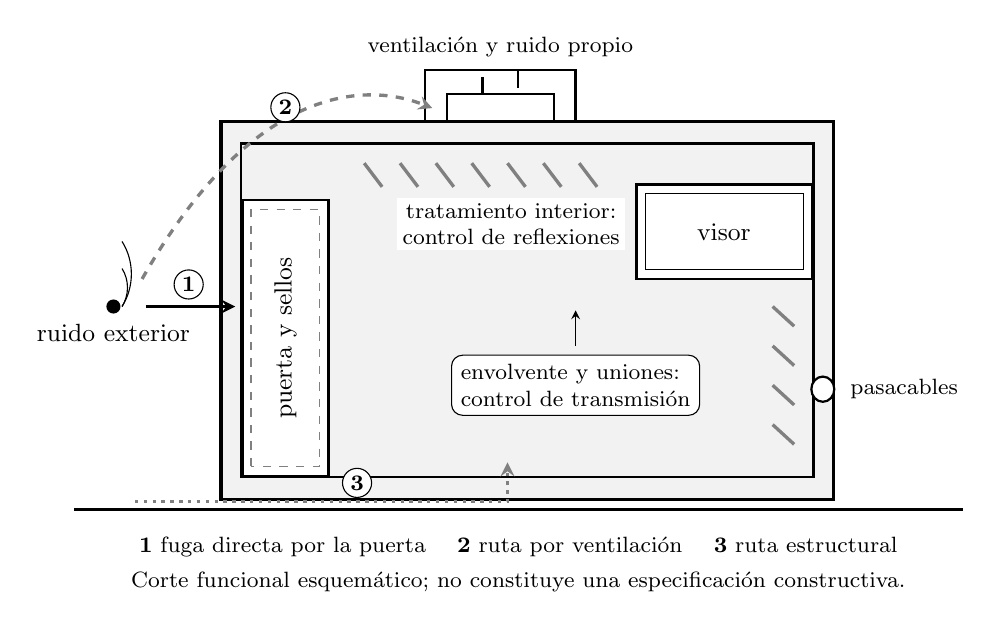
\begin{tikzpicture}[
    x=0.91cm,
    y=1cm,
    >=stealth,
    font=\small,
    directa/.style={very thick,->},
    lateral/.style={very thick,gray,dashed,->},
    estructural/.style={very thick,gray,dotted,->},
    marca/.style={draw,circle,fill=white,inner sep=1.2pt,font=\footnotesize\bfseries}
]
    % Envolvente doble y base
    \path[fill=black!5] (2.20,0.75) rectangle (10.75,5.55);
    \draw[very thick] (2.20,0.75) rectangle (10.75,5.55);
    \draw[thick] (2.48,1.03) rectangle (10.47,5.27);
    \draw[very thick] (0.15,0.62) -- (12.55,0.62);

    % Puerta y sello
    \path[fill=white] (2.50,1.05) rectangle (3.70,4.55);
    \draw[thick] (2.50,1.05) rectangle (3.70,4.55);
    \draw[gray,dashed] (2.62,1.17) rectangle (3.58,4.43);
    \node[rotate=90] at (3.10,2.80) {puerta y sellos};

    % Visor
    \path[fill=white] (8.00,3.55) rectangle (10.45,4.75);
    \draw[thick] (8.00,3.55) rectangle (10.45,4.75);
    \draw[thin] (8.12,3.67) rectangle (10.33,4.63);
    \node at (9.22,4.15) {visor};

    % Tratamiento interior
    \foreach \x in {4.20,4.70,5.20,5.70,6.20,6.70,7.20}{
        \draw[very thick,gray] (\x,5.02) -- (\x+0.25,4.72);
    }
    \foreach \y in {1.45,1.95,2.45,2.95}{
        \draw[very thick,gray] (10.20,\y) -- (9.90,\y+0.25);
    }
    \node[align=center,font=\footnotesize,fill=white,inner sep=2pt]
        at (6.25,4.25)
        {tratamiento interior:\\control de reflexiones};

    % Conducto de ventilación con dos cambios de dirección
    \draw[thick] (5.05,5.55) -- (5.05,6.20) -- (7.15,6.20) -- (7.15,5.55);
    \draw[thick] (5.35,5.55) -- (5.35,5.90) -- (6.85,5.90) -- (6.85,5.55);
    \draw[thick] (5.85,5.90) -- (5.85,6.12);
    \draw[thick] (6.35,5.98) -- (6.35,6.20);
    \node[anchor=south,font=\footnotesize] at (6.10,6.25)
        {ventilación y ruido propio};

    % Pasacables
    \draw[thick,fill=white] (10.60,2.15) circle (0.16);
    \node[anchor=west,font=\footnotesize] at (10.85,2.15) {pasacables};

    % Fuente exterior y trayectorias
    \node[fill=black,circle,inner sep=1.8pt] (s) at (0.70,3.20) {};
    \node[anchor=north] at (s.south) {ruido exterior};
    \draw (0.82,3.20) arc (-35:35:0.42);
    \draw (0.82,3.20) arc (-35:35:0.72);

    \draw[directa] (1.15,3.20) -- (2.40,3.20);
    \node[marca] at (1.75,3.48) {1};
    \draw[lateral] (1.10,3.55)
        .. controls (2.60,5.95) and (4.15,6.08) .. (5.15,5.72);
    \node[marca] at (3.10,5.73) {2};
    \draw[estructural] (1.00,0.72) -- (6.20,0.72) -- (6.20,1.22);
    \node[marca] at (4.10,0.96) {3};

    \node[draw,rounded corners,fill=white,align=left,font=\footnotesize]
        at (7.15,2.20)
        {envolvente y uniones:\\control de transmisión};
    \draw[->] (7.15,2.70) -- (7.15,3.15);

    \node[font=\footnotesize,anchor=north,text width=11cm,align=center]
        at (6.35,0.40)
        {\textbf{1} fuga directa por la puerta \quad
         \textbf{2} ruta por ventilación \quad
         \textbf{3} ruta estructural};
    \node[font=\footnotesize,anchor=north] at (6.35,-0.05)
        {Corte funcional esquemático; no constituye una especificación constructiva.};
\end{tikzpicture}
